\capitulo{5}{Aspectos relevantes del desarrollo del proyecto}

\section{Metodologías Aplicadas}

Desde el inicio del proyecto se tenía muy claro que se iba a proceder de la manera más ordenada y profesional posible. Para poder realizar exitosamente este proceso recurrimos a diferentes herramientas que nos permitiesen realizar un correcto desarrollo de este proyecto.

A continuación se comentan las herramientas utilizadas:
\begin{itemize}
    \item Kanban:
\end{itemize}
 La metodología Kanban consiste en poder informarte del estado de las tareas del proyecto de una forma visual y rápida, por lo que, con una rápida visualización, podemos saber el estado de cada una de las tareas existentes en el tablero.

 \begin{figure}[h]
     \centering
     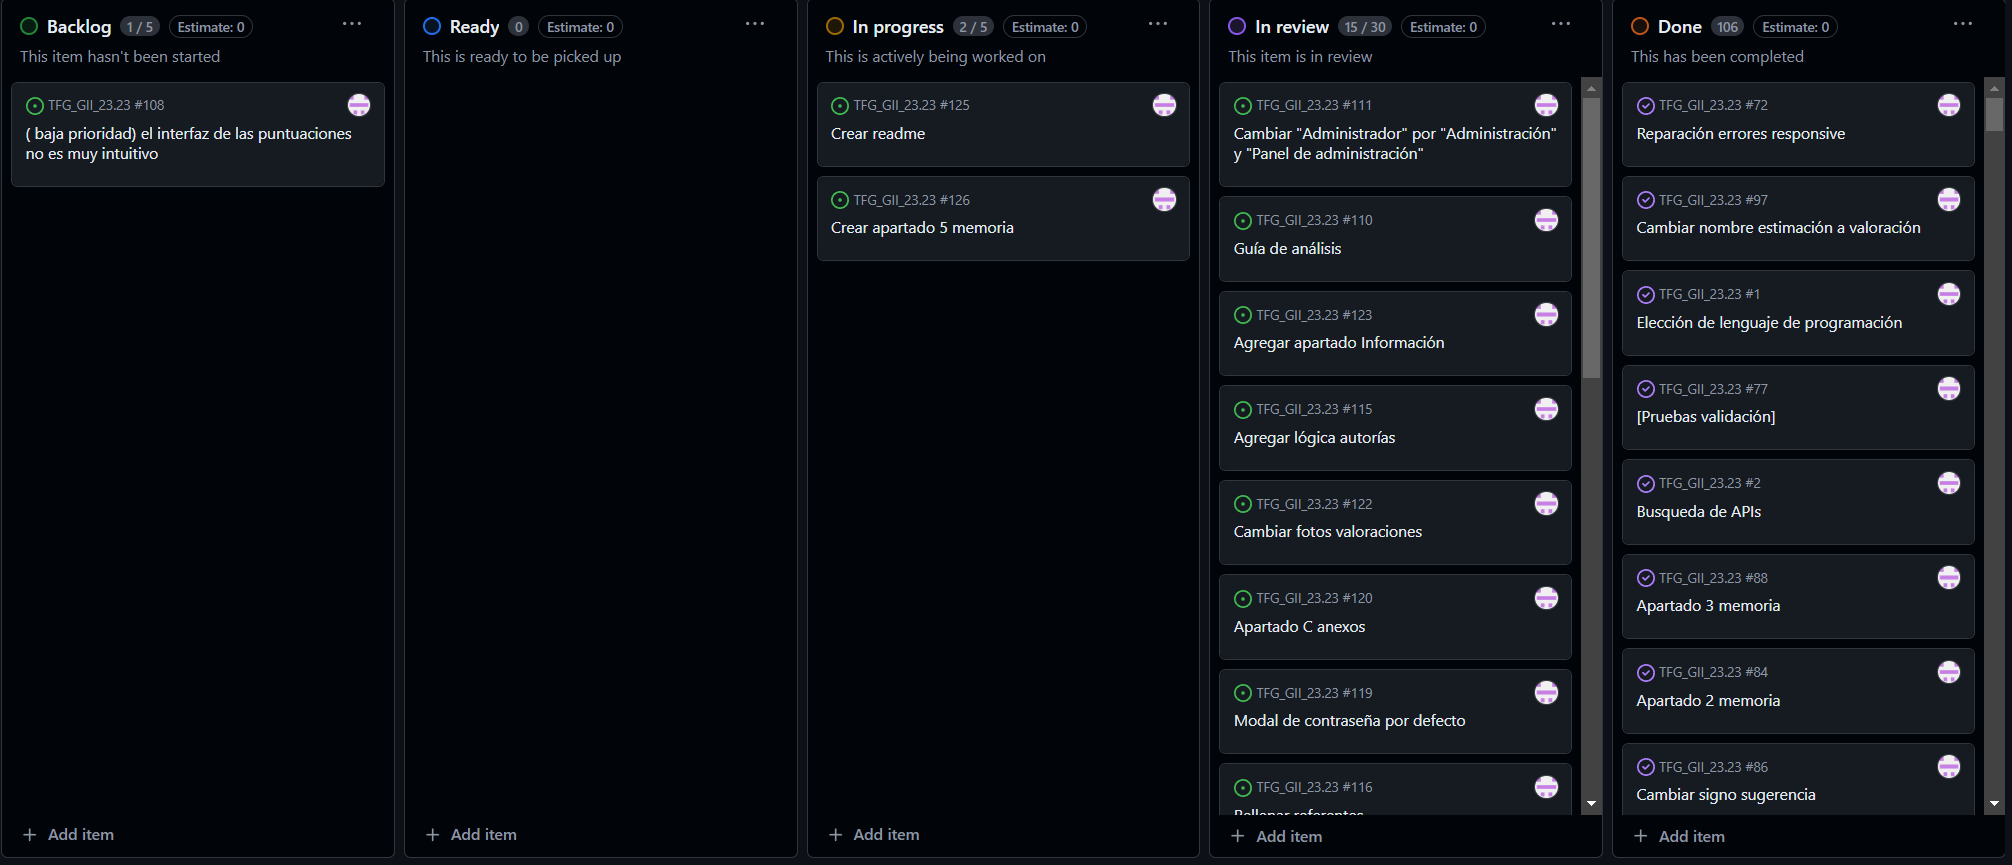
\includegraphics[width=1\linewidth]{Imagenes/Tablero kanban.png}
     \caption{Tablero Kanban}
     \label{Tablero Kanban}
 \end{figure}
 \FloatBarrier
 \begin{itemize}
     \item Scrum
 \end{itemize}
Esta metodología principalmente se posiciona en realizar ciclos de trabajos (Sprints) con una duración fija, en la que al finalizar se realiza una entrega del proyecto. Esto permite tener una mayor flexibilidad durante el proyecto y una correcta entrega continua que nos permite la máxima colaboración con el cliente, en este caso el profesor de la UBU Jesús Alberto San Martín Zapatero~\cite{PerfilJesus}.
En este caso se han realizado Sprints de 2 semanas con una reunión al finalizar el Sprint para poder debatir acerca de la entrega realizada y realizar las propuestas de trabajo para el siguiente Sprint.
Una vez generadas esas propuestas se transformaban en tareas que se incluían en el tablero Kanban para realizar un seguimiento a tiempo real del progreso del Sprint.

\section{Formación}
Para la realización del proyecto han sido necesarios diferentes conocimientos técnicos para poder plasmar las ideas y los prototipos en una aplicación web real y completa. Dentro de todos estos conocimientos requeridos, existían algunos de ellos que no se disponían al iniciar el proyecto, por ese motivo, se dedicó tiempo a realizar formaciones sobre los siguientes elementos:
\begin{itemize}
    \item Flask: Aunque Flask sea un Framework de Python, contiene elementos y bibliotecas compatibles que agregan funcionalidades muy distintas a lo existente en una versión nativa de Python.
    Para poder hacer frente a la necesidad de estos nuevos conocimientos, se ha utilizado la documentación de Flask~\cite{Flask} de manera principal para poder tener un punto de partida sólido y unas directrices básicas. Tras tener los puntos esenciales, a través de diferentes videos y pequeños cursos se realizaron pequeños proyectos de prueba para ir desarrollando las habilidades necesarias.

    \item Angular: Angular es una herramienta que de manera inicial no se encontraba contemplada en este proyecto, sin embargo, tras mi experiencia en las prácticas curriculares y la posibilidad de realizar un curso profesional de Angular~\cite{CursoAngular}, se presentó como una opción muy interesante para aumentar la complejidad de la aplicación web y disponer de más herramientas para el desarrollo del \textit{Frontend}, así como numerosas ventajas para la parte de diseño del proyecto, permitiendo crear una web más rápida y fácilmente reutilizable y escalable. 
    Como Angular es un Framework, este curso aportó conocimientos de TypeScript, HTML y CSS.
\end{itemize}

\section{Inicio del proyecto}
Esta idea comenzó por parte del profesor de la UBU Jesús Alberto San Martín Zapatero con el afán de aportar una nueva herramienta que permitiese a docentes y familias realizar consultas acerca de la rigurosidad científica existente en términos de perspectiva de género de los libros de la prehistoria. 

Este proyecto tiene como nombre PREHISTORIA EN IGUALDAD.
\begin{figure}[h]
    \centering

\includegraphics[width=0.5\linewidth]{Imagenes/Logo.png}
    \caption{Logo de la web}
    \label{Logo de la web}
\end{figure}
\FloatBarrier

Para poder plasmar esa idea en un proyecto real, se puso en contacto con la facultad de Informática y comenzamos con el desarrollo de esa aplicación web.

Una de las partes positivas de este proyecto ha sido la posibilidad de realizarlo tratando con el docente mencionado como si fuera un cliente al que entregar un producto, lo cuál también ha sido un reto añadido en este proyecto. Esto ha aportado valor al desarrollo ya que a lo largo de cada pequeña entrega se han tenido que realizar demostraciones del programa y trasladar los requisitos necesarios propuestos por él a un producto viable.

Una vez decidido el comienzo del proyecto, se llegó al acuerdo de utilizar el Framework de python Flask como \textit{frontend} y \textit{backend} de la aplicación, y se desarrollaron prototipos básicos como la imagen de debajo, permitiendo dar una idea de cómo podría quedar la aplicación una vez desarrollada.

\begin{figure}[h]
    \centering
    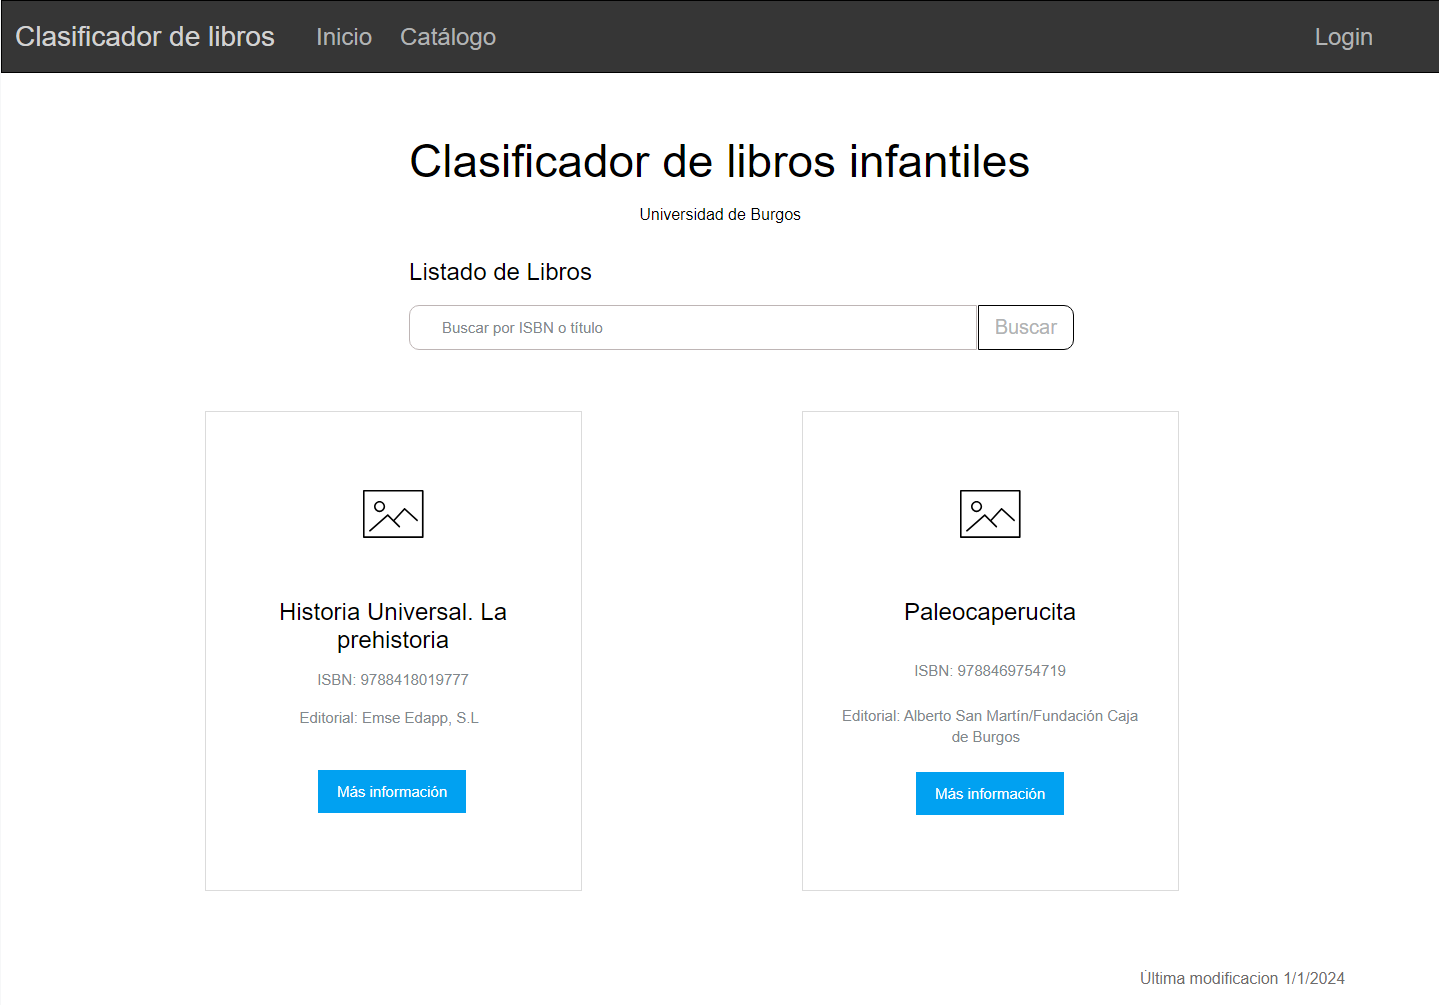
\includegraphics[width=0.8\linewidth]{Imagenes/PrototipoCatalogo.png}
    \caption{Prototípo del catálogo}
    \label{Prototípo del catálogo}
\end{figure}
\FloatBarrier


\section{Desarrollo del \textit{frontend}}
Al comienzo del desarrollo, como ya se ha mencionado, se ha utilizado el \textit{framework} Flask, el cuál permite realizar conexiones directas entre el \textit{frontend} y el \textit{backend} mediante funciones muy simples. Además de este \textit{framework}, se utilizó bootstrap~\cite{Bootstrap5}, el cuál es un \textit{toolkit} disponible para numerosos lenguajes que permite obtener de una manera rápida componentes prediseñados que facilitan el desarrollo en HTML y CSS.
Tras realizar diversos desarrollos entre los que se encontraba el catálogo con sus opciones de edición protegido por un inicio de sesión, se fueron incluyendo más ideas de desarrollo para poder ampliar la aplicación y permitir a los usuarios tener su propia estimación de un libro.

Uno de los mayores problemas de este desarrollo consistió en la dependencia que existía entre \textit{front} y \textit{back}. Esto podía generar un problema en el caso de que una de las dos partes fallase, impidiendo al usuario utilizar la funcionalidad que funcionase correctamente. La solución adoptada consistió en separar ambas partes para brindar total independencia. Esto se traduce en que por ejemplo, si se diese el caso de que el \textit{backend} fallase, la interfaz del usuario podría seguir mostrando al usuario la información que desease pero de forma limitada, reduciendo así las posibilidades de que todo el conjunto falle y de ninguna forma un usuario pueda interactuar con la aplicación.

Para aplicar la solución encontrada, se decidió refactorizar el proyecto entero a un sistema cliente-servidor utilizando los \textit{frameworks} Angular y Flask. Esta decisión se consolidó debido a la posibilidad de realizar un curso de pago y el conocimiento adquirido durante las prácticas curriculares.


Esta refactorización supuso un antes y un después en el diseño del proyecto y su rendimiento, ya que Angular, al ser un SPA, no tiene que cargar página a página, sino que tiene todos sus componentes cargados y los va mostrando u ocultando en función de la interacción del usuario. Por lo tanto, mereció la pena retrasar un poco la planificación inicial dados los resultados obtenidos.

Además, se dejó de aplicar Bootstrap 5~\cite{Bootstrap5} y se comenzó a utilizar PrimeNG~\cite{PrimeNG} y PrimeIcons~\cite{PrimeIcons} para la generación de componentes con responsive incluido y sweetAlert2 para las ventanas modales de confirmación u avisos.

Estas nuevas herramientas han permitido desarrollar una aplicación web mucho mas compleja y dinámica para que tanto usuarios como el personal de administración puedan interactuar con una gran variedad de opciones a su disposición.

La tarea para realizar esto fue de gran complejidad ya que se rediseñó toda la estructura de los ficheros y la gran mayoría del HTML no se podía reutilizar por el uso de Bootstrap, por lo que se reprogramó todo lo hecho hasta ese desarrollo mientras, paralelamente, se continuaba en Flask por si el resultado de la refactorización no era satisfactorio. 


Una vez realizada completamente la refactorización, se rediseñó la interfaz del personal de administración, el cual en la anterior versión únicamente permitía hacer modificaciones del catálogo y realizar importaciones o exportaciones desde el propio catálogo. El sistema de gestión de usuarios se realizaba a nivel de código, por lo que no era útil para la administración.

\begin{figure}[h]
    \centering
    
\includegraphics[width=0.9\linewidth]{Imagenes/administracionAntiguo.png}
    \caption{Administración antígua}
    \label{Administración antígua}
\end{figure}
\FloatBarrier

Tras los desarrollos pedidos por el cliente, los cuales se centraban en mostrar información al usuario sobre los libros estimados por el personal de administración, las estimaciones de los propios usuarios y recomendaciones de recursos para facilitar el aprendizaje, se iban desarrollando paralelamente elementos los cuales permitían automatizar y personalizar la aplicación web de manera gráfica y sencilla desde una panel de administración completo.

\begin{figure}[h]
    \centering
    
\includegraphics[width=0.5\linewidth]{Imagenes/PanelAdmin.png}
    \caption{Panel de Administración}
    \label{Panel de Administración}
\end{figure}
\FloatBarrier

\section{Desarrollo del \textit{backend}}
Esta parte de la aplicación, a diferencia del \textit{frontend}, no ha sufrido un cambio de tecnología, simplemente se ha cambiado el esquema de los archivos y se han modificado las funciones para poder funcionar como una API y poder conectarse satisfactoriamente con el Angular. De manera adicional, al generar esta separación, se pueden realizar llamadas a este servicio sin la necesidad de Angular, a través de aplicaciones como Postman~\cite{Postman}. Esto deja una puerta abierta a la posibilidad de distribución de la API para que puedan trabajar con ellos terceros e implementarlo en sus sistemas.

Durante el diseño de esta API se decidió separar por grupos funcionales todas las funciones de la aplicación, pudiendo así incorporar nuevas utilidades de forma sencilla sin tener que modificar otras funciones.

\begin{figure}[h]
    \centering
    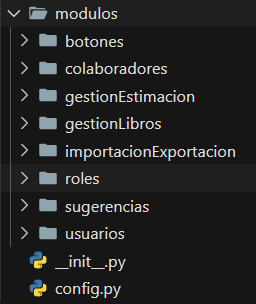
\includegraphics[width=0.5\linewidth]{Imagenes/Modulos.png}
    \caption{Módulos del proyecto}
    \label{Módulos del proyecto}
\end{figure}
\FloatBarrier

Dentro de esta API se encuentran todas las funcionalidades existentes para un correcto funcionamiento de todos los requisitos funcionales mencionados en los anexos.
Estas funciones dependen de una base de datos donde se guarda toda la información utilizada por la aplicación web.

\subsection{Web scraping}
El web sraping de esta aplicación tiene como origen la propuesta de facilitar la búsqueda de libros utilizando diferentes fuentes bibliográficas, utilizando la API de Google Books y las otras dos son páginas web:
\begin{itemize}
    \item Amazon
    \item Agapea
\end{itemize}

El inicio de este requisito comienza al recibir en el backend una petición adjuntando un identificador del libro que que desea (Título, ISBN10 o ISBN13). 

Una vez estos datos llegan al \textit{backend}, se llama a una función auxiliar encargada de realizar las llamadas a las fuentes. Como dependiendo del parámetro pasado inicialmente por el equipo de administración puede influir en los pasos a seguir en la fuente de Agapea y en la fuente de Google Books, como primera tarea a realizar es identificar mediante expresiones regulares si se trata de un ISBN o de un título. Para esto se utiliza la función buscar\_libro.

\begin{figure}[h]
    \centering
    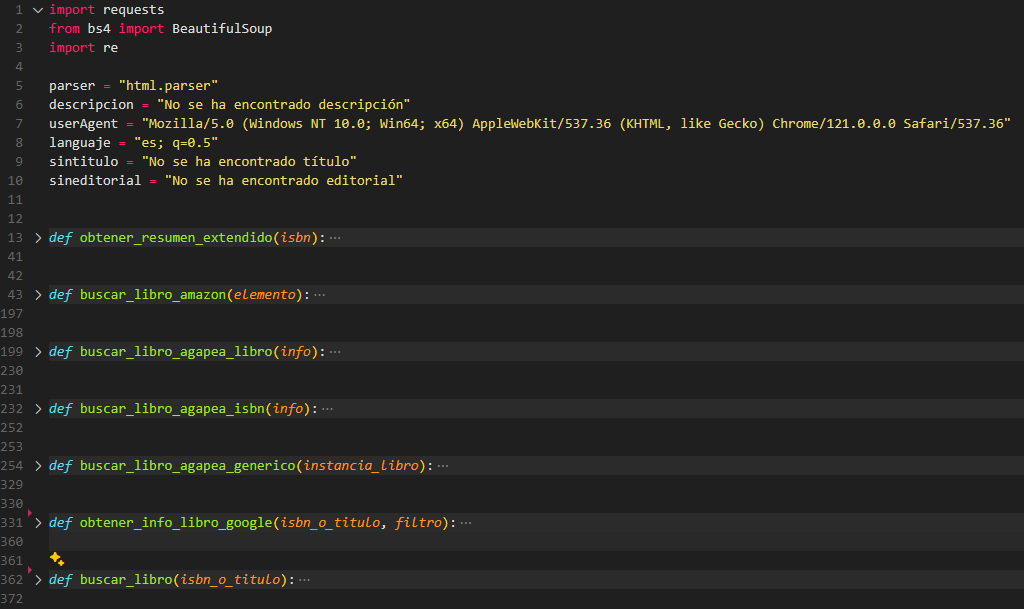
\includegraphics[width=1\linewidth]{Imagenes/Funciones web scraping.png}
    \caption{Funciones web scraping}
    \label{Funciones web scraping}
\end{figure}
\FloatBarrier

\subsubsection{Web scraping Agapea}
Para esta primera fuente, la manera de buscar los libros varía significativamente, ya que si el usuario introduce el ISBN, si se incluye el ISBN en la URL de la web nos va a llevar directamente a la ficha del libro, mientras que si se busca por título, primero es necesario acceder a un listado de libros con resultados que podrían equivaler al texto introducido y después entrar en la ficha del libro.

Para realizar esos pasos diferentes se crearon dos funciones las cuales cada una se encargaba de un tipo de búsqueda. Al finalizar la ejecución, ambas funciones llaman a una función común que se encarga de recopilar la información disponible en la ficha del libro.


Uno de los mayores problemas que se generaron al trabajar con esta fuente es que el contenido del Resumen en la ficha del libro está limitado por un Leer Más tal como aparece en la figura \ref{Leer Más Agapea}.


\begin{figure}[h]
    \centering
    
\includegraphics[width=1\linewidth]{Imagenes/leerMasAgapea.png}
    \caption{Leer Más Agapea}
    \label{Leer Más Agapea}
\end{figure}
\FloatBarrier


Para poder solucionar este limitante, se estudió la arquitectura de la página y se descubrió que realizando una solicitud Ajax~\cite{Ajax} al servidor de Agapea se podía indicar a la web que se deseaba leer toda la información y posteriormente recoger los datos. La llamada se puede detectar en la web al inspeccionarla en el apartado network.

Una solicitud Ajax es una técnica que se utiliza para enviar y recibir datos de un servidor sin necesidad de recargar la web utilizando mayoritariamente Javascript y XML de manera asíncrona.

\begin{figure}[h]
    \centering
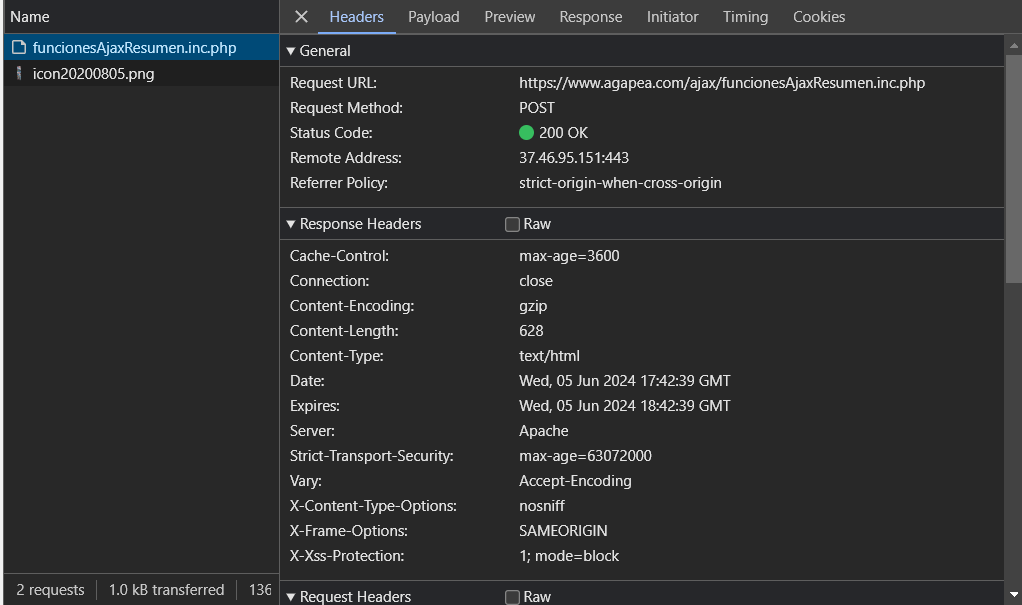
\includegraphics[width=0.9\linewidth]{Imagenes/AgapeaAjax.png}
    \caption{Función Ajax Agapea}
    \label{Función Ajax Agapea}
\end{figure}
\FloatBarrier

\subsubsection{ Web scraping Amazon}
Para esta segunda fuente no es necesaria esa distinción entre ISBN y título, ya que ambos elementos redirigen a un menú donde se puede seleccionar el producto deseado. 

Una vez obtenido la ficha del libro, se van haciendo comprobaciones para consolidar la existencia de los datos y poder almacenarlos. En el caso de que no se encuentre alguno de los datos, se incluye en el resultado como "No se ha encontrado el elemento X".

\subsubsection{API Google Books}
Esta tercera y última fuente se obtiene directamente realizando llamadas a una API propiedad de Google. Esta API nos pide una distinción entre ISBN y título, por lo que es necesario pasárselo por parámetro para realizar la llamada.
Debido al tipo de llamada que vamos a realizar, el cuál apunta al \textit{endpoint} correspondiente al apartado volúmenes, no es necesario registrarse ni tener un token de autenticación, esto nos permite realizar llamadas sin un limite establecido a cualquier tipo de libro.
Tras realizar la llamada al \textit{endpoint} indicándole el título o el ISBN, la API devuelve la información que contiene en un JSON, por lo que se traduce y se comprueba la existencia de datos válidos en esa respuesta.

Como esta es la última función en ejecutarse, al finalizar devuelve el control a la función principal que recoge el resultado de todas las fuentes y las guarda en una base de datos temporal para que el equipo de administración decida si utiliza esos datos obtenidos y de que manera (Escogiendo una única fuente o combinando varias de ellas).


\subsection{Gestión de permisos}
Tras ir haciendo desarrollos se presentó la idea de no permitir a todos los miembros del equipo de administración realizar todas las gestiones disponibles en el \textit{frontend}, sino que dependiendo del usuario se le bloquease o desbloquease las funcionalidades dinámicamente. Para la resolución de ese problema, además de existir una cuenta por usuario, se creó un sistema de roles dinámicos con permisos. Es decir, los miembros del equipo de administración que tengan los permisos necesarios, pueden crear, editar y eliminar todos los roles que necesiten tener en la aplicación, y establecer a cada uno de esos roles una serie de permisos activados y desactivados.

Esto significa que cuando el \textit{frontend} quiere cambiar de pestaña, manda una solicitud de permisos al \textit{backend} preguntando si ese usuario tiene los permisos necesarios para poder acceder a ese recurso, la función responsable de esa parte revisa sus credenciales y devuelve una respuesta afirmativa o negativa para que le muestre la pestaña si es admitido, o una modal indicándole que no tiene permisos para realizar esa acción.

\begin{figure}[h]
    \centering
    
\includegraphics[width=0.75\linewidth]{Imagenes/Modal sin permiso.png}
    \caption{Modal Usuario sin Permisos}
    \label{Modal Usuario sin Permisos}
\end{figure}
\FloatBarrier


\section{Despliegue de la aplicación}
Para desplegar esta aplicación, se utilizaron dos plataformas diferentes:
\begin{itemize}
    \item Netlify para el \textit{frontend}.
    \item Render para el \textit{backend}.
\end{itemize}

Netlify~\cite{Netlify} es una plataforma de despliegue para sitios web compatible con Angular. Esta herramienta cuenta con un plan gratuito con el que se puede subir el proyecto desde Github. 
Aunque esta herramienta esta pensada para esta tecnología, durante el proceso de despliegue aparecieron problemas relativos a las redirecciones de la aplicación. Esto se debe a que Netlify intenta cargar esa URL pero no encuentra nada. Esto se debe a que Angular es un SPA, por lo que no tienen que existir redirecciones con la carga de nuevo de la página. Para poder solucionar este problema correctamente, al crear los ficheros de producción del \textit{frontend}, se necesitó añadir un archivo que indica a Netlify que las redirecciones siempre lleven a la pantalla principal aunque cambie de URL.

Una gran ventaja que aporta esta herramienta es la realización de actualizaciones automáticas de la web. Es decir, cada vez que detecta un cambio en el repositorio de Github automáticamente comienza a construir la nueva versión mientras mantiene activa la antigua, una vez la más actualizada está preparada, sustituye una por otra, permitiendo así el máximo tiempo de disponibilidad posible en la aplicación web. En el caso de que detecte un cambio pero no pertenezca al \textit{frontend}, no realiza esta acción. 

La interfaz gráfica de Netlify es muy visual y sencilla, teniendo un apartado de \textit{deploys} donde marca el estado de construcción del sitio al incorporar nuevos cambios.

En la figura \ref{Interfaz Deploys Netlify} se puede observar los últimos despliegues realizados en este servicio, en los cuales se puede entrar para ver la información relativa a ese despliegue y la posibilidad de forzar esa versión como la más actualizada.

\begin{figure}[h]
    \centering
    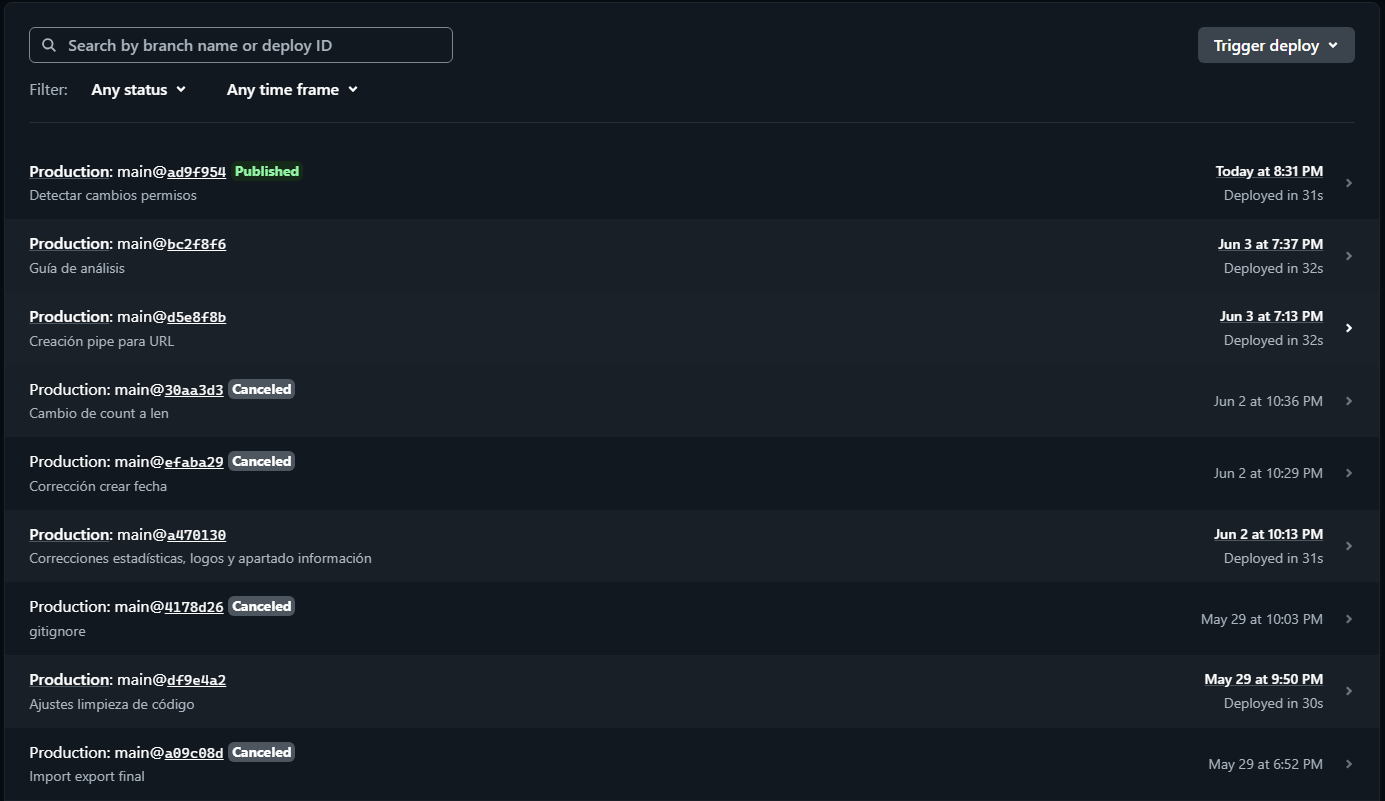
\includegraphics[width=1\linewidth]{Imagenes/Interfaz Netlify.png}
    \caption{Interfaz Deploys Netlify}
    \label{Interfaz Deploys Netlify}
\end{figure}
\FloatBarrier

Por otra parte, Render ha sido la herramienta elegida para realizar el despliegue del \textit{backend} Flask. Render, a diferencia de Netlify es más global y acepta diferentes tipos de despliegues. 
Esta herramienta se ha usado para el despliegue utilizando la opción de web service inicialmente con una cuenta gratuita. Una vez conectado con el repositorio de Github y establecidas las carpetas y comandos de arranque se desplegó la aplicación con las mismas características de autodespliegue que Netlify. 


\begin{figure}[h]
    \centering
    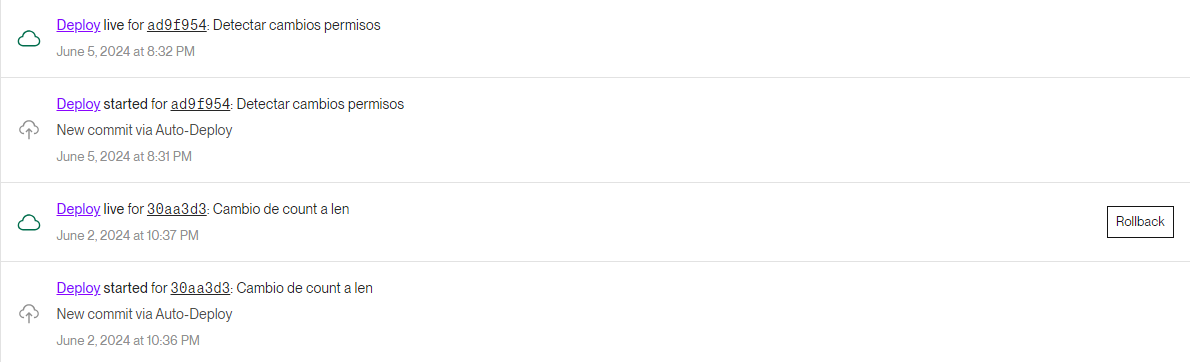
\includegraphics[width=0.9\linewidth]{Imagenes/DeploysRender.png}
    \caption{Pantalla Deploys Render}
    \label{Pantalla Deploys Render}
\end{figure}
\FloatBarrier


Para los ficheros de configuración que pueden contener contenido sensible, se migraron esos datos al apartado de variables de entorno para aumentar la seguridad cifrándolas y guardándolas de forma aislada.

\begin{figure}[h]
    \centering
    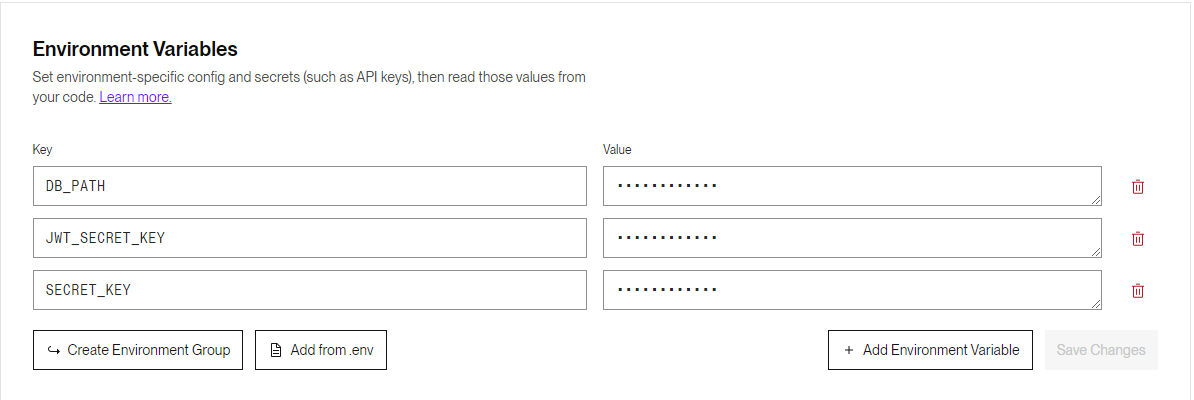
\includegraphics[width=0.9\linewidth]{Imagenes/RenderENV.png}
    \caption{Variables de entorno Render}
    \label{Variables de entorno Render}
\end{figure}
\FloatBarrier

Tras el despliegue y el inicio de realización de pruebas, se detectó que la base de datos al encontrarse integrada, al cerrarse el servidor se borraban todos los datos que no se encontrasen añadidos desde el \textit{commit}. Para solucionar esto ha sido necesario pagar la versión más barata de este servicio para poder tener un disco dedicado a la base de datos y un servidor 24 horas encendido. 

Para subir la base de datos al disco de Render, se necesitó realizar una conexión SSH utilizando unas claves dadas por Render para poder acceder remotamente al sistema de ficheros y poder enviar a esa dirección la base de datos que contenía los datos mínimos para funcionar correctamente.


\section{Testing}
El proceso de testing es una parte fundamental del desarrollo de software que asegura la calidad y fiabilidad del producto final. En este proyecto, se han realizado pruebas unitarias para verificar el correcto funcionamiento de los diferentes componentes de la aplicación web.

\subsection{Pruebas Unitarias}
Las pruebas unitarias se implementaron utilizando el framework \texttt{unittest}~\cite{Unittest} de Python. Este framework permite definir y ejecutar pruebas para asegurar que las funciones y métodos individuales se comporten como se espera. Cada prueba verifica una pequeña unidad de funcionalidad de forma aislada, permitiendo identificar y corregir errores de manera temprana en el ciclo de desarrollo.

Las pruebas unitarias son cruciales por varias razones:
\begin{itemize}
    \item \textbf{Aseguran la calidad del código}: Verifican que cada función y método produce los resultados esperados para los \textit{inputs} establecidos. Esto ayuda a identificar errores en la lógica antes de que se integren en la versión de producción.
    \item \textbf{Facilitan el \textit{Refactoring}}: Permiten realizar cambios en el código con la confianza de que no se introducirán errores. Si una prueba unitaria falla después de un cambio, el equipo de desarrollo sabe exactamente qué parte del código fue afectada.
    \item \textbf{Documentación del Código}: Las pruebas unitarias sirven como una forma de documentación que explica cómo se espera que el código se comporte. Esto es especialmente útil para nuevos el equipo de desarrollo que se integran al proyecto.
    \item \textbf{Detección Temprana de Errores}: Al identificar problemas en las primeras etapas del desarrollo, se reduce el coste y tiempo de corrección. Es más económico y rápido corregir errores encontrados durante el desarrollo que aquellos encontrados después del despliegue.
\end{itemize}

\subsection{Proceso de Testing}
El proceso de testing en este proyecto sigue una metodología sistemática para asegurar que todas las funcionalidades sean probadas de manera exhaustiva. Los pasos incluyen:

\begin{itemize}
    \item \textbf{Implementación de Pruebas}: Utilizando \texttt{unittest}, se implementan las pruebas correspondientes para cada caso de prueba que se considere crítico.
    \item \textbf{Ejecución de Pruebas}: Las pruebas se ejecutan regularmente durante el desarrollo para asegurar que cualquier cambio en el código no introduce nuevos errores. Esto se logra mediante la ejecución de todas las pruebas unitarias como parte del ciclo de desarrollo continuo.
    \item \textbf{Análisis de Resultados}: Los resultados de las pruebas son analizados para identificar y corregir errores. Cualquier falla en una prueba unitaria indica un problema que debe ser investigado y resuelto.
\end{itemize}

\subsection{Beneficios Generales del Testing}
El testing en general ofrece varios beneficios clave en el desarrollo de software:
\begin{itemize}
    \item \textbf{Mejora de la Calidad del Código}: A través de pruebas rigurosas, se garantiza que el código cumple con los estándares de calidad y se comporta como se espera.
    \item \textbf{Reducción de Costos}: Identificar y corregir errores durante el desarrollo es mucho menos costoso que hacerlo después de que el software ha sido desplegado.
    \item \textbf{Mantenimiento Sostenible}: El código bien probado es más fácil de mantener y actualizar, ya que las pruebas ayudan a identificar rápidamente los impactos de los cambios.
\end{itemize}


\section{Uso de Postman}

Postman es una herramienta para el desarrollo de APIs que facilita la creación, el envío y el análisis de solicitudes HTTP. En este proyecto, se utilizó Postman para realizar pruebas manuales de la API desarrollada.

\subsection{Pruebas Manuales}
Las pruebas manuales con Postman implican el envío de solicitudes HTTP a los endpoints de la API y la verificación de las respuestas. Esto es útil para:
\begin{itemize}
    \item \textbf{Verificación Rápida}: Permite al equipo de desarrollo verificar rápidamente la funcionalidad de los endpoints durante el desarrollo. Se pueden enviar solicitudes GET, POST, PUT, DELETE, entre otras, para comprobar las respuestas de la API.
    \item \textbf{Depuración}: Ayuda a identificar y resolver problemas en las API de manera interactiva. El equipo de desarrollo puede ajustar los parámetros de las solicitudes y observar cómo cambian las respuestas.
    \item \textbf{Exploración}: Facilita la exploración de las funcionalidades de la API y el ensayo de diferentes casos de uso. Esto es especialmente útil durante la fase de desarrollo para entender cómo interactúan diferentes partes de la API.
\end{itemize}

Para llevar a cabo las pruebas manuales con Postman, se siguen los siguientes pasos:

\begin{enumerate}
    \item \textbf{Configuración de la Solicitud}: Se selecciona el tipo de solicitud HTTP (GET, POST, PUT, DELETE) y se especifica la URL del endpoint que se desea probar.
    \item \textbf{Configuración de los Parámetros}: Si la solicitud requiere parámetros, estos se configuran en la sección correspondiente de Postman. Esto puede incluir parámetros de URL, headers, y cuerpo de la solicitud en formato JSON.
    \item \textbf{Envio de la Solicitud}: Se envía la solicitud y se espera la respuesta del servidor. Postman muestra la respuesta en su interfaz, incluyendo el código de estado HTTP, los headers de la respuesta y el cuerpo de la respuesta.
    \item \textbf{Verificación de la Respuesta}: Se verifica que la respuesta del servidor sea la esperada. Esto incluye comprobar que el código de estado HTTP es correcto y que el cuerpo de la respuesta contiene los datos esperados.
\end{enumerate}
 
\begin{figure}[h]
    \centering
    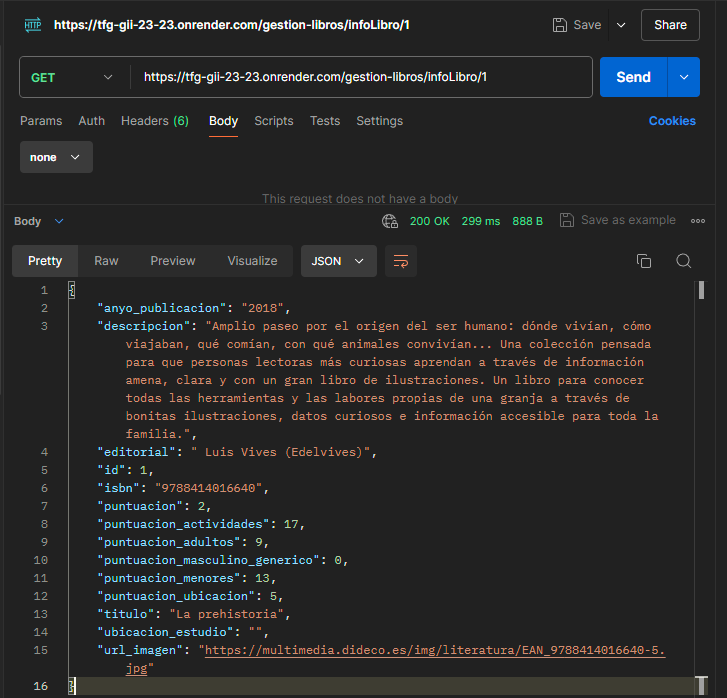
\includegraphics[width=0.7\linewidth]{Imagenes/PostmanEjemplo.png}
    \caption{Ejemplo llamada con Postman}
    \label{Ejemplo llamada con Postman}
\end{figure}
\FloatBarrier